% Autor: Leonhard Segger, Alexander Neuwirth
% Datum: 2017-10-30
\documentclass[
	% Papierformat
	a4paper,
	% Schriftgröße (beliebige Größen mit „fontsize=Xpt“)
	12pt,
	% Schreibt die Papiergröße korrekt ins Ausgabedokument
	pagesize,
	% Sprache für z.B. Babel
	ngerman
]{scrartcl}

% Achtung: Die Reihenfolge der Pakete kann (leider) wichtig sein!
% Insbesondere sollten (so wie hier) babel, fontenc und inputenc (in dieser
% Reihenfolge) als Erstes und hyperref und cleveref (Reihenfolge auch hier
% beachten) als Letztes geladen werden!

\usepackage{tikz}
\usetikzlibrary{calc,patterns,angles,quotes} % loads some tikz extensions\usepackage{tikz}
\usetikzlibrary{babel}

% Silbentrennung etc.; Sprache wird durch Option bei \documentclass festgelegt
\usepackage{babel}
% Verwendung der Zeichentabelle T1 (Sonderzeichen etc.)
\usepackage[T1]{fontenc}
% Legt die Zeichenkodierung der Eingabedatei fest, z.B. UTF-8
\usepackage[utf8]{inputenc}
% Schriftart
\usepackage{lmodern}
% Zusätzliche Sonderzeichen
\usepackage{textcomp}

% Mathepaket (intlimits: Grenzen über/unter Integralzeichen)
\usepackage[intlimits]{amsmath}
% Ermöglicht die Nutzung von \SI{Zahl}{Einheit} u.a.
\usepackage{siunitx}
% Zum flexiblen Einbinden von Grafiken (\includegraphics)
\usepackage{graphicx}
% Abbildungen im Fließtext
\usepackage{wrapfig}
% Abbildungen nebeneinander (subfigure, subtable)
\usepackage{subcaption}
% Funktionen für Anführungszeichen
\usepackage{csquotes}
\MakeOuterQuote{"}
% Zitieren, Bibliografie
\usepackage[sorting=none]{biblatex}


% Zur Darstellung von Webadressen
\usepackage{url}
%chemische Formeln
\usepackage[version=4]{mhchem}
% siunitx: Deutsche Ausgabe, Messfehler getrennt mit ± ausgeben
\usepackage{floatrow}
\floatsetup[table]{capposition=top}
\usepackage{float}
% Verlinkt Textstellen im PDF-Dokument
\usepackage[unicode]{hyperref}
% "Schlaue" Referenzen (nach hyperref laden!)
\usepackage{cleveref}
\sisetup{
	locale=DE,
	separate-uncertainty
}
\bibliography{BA-C-04_V05_08-04-2019_References}

\begin{document}

	\begin{titlepage}
		\centering
		{\scshape\LARGE Versuchsbericht zu \par}
		\vspace{1cm}
		{\scshape\huge V05 - Lebensdauermessung eines $\gamma$-Niveaus \par}
		\vspace{2.5cm}
		{\LARGE Gruppe BA-C-04 \par}
		\vspace{0.5cm}

		{\large Alexander Neuwirth (E-Mail: a\_neuw01@wwu.de) \par}
		{\large Leonhard Segger (E-Mail: l\_segg03@uni-muenster.de) \par}
		\vfill

		durchgeführt am 08.04.2019\par
		betreut von\par
		{\large Daniel Guderian}
		\vfill

		{\large \today\par}
	\end{titlepage}
	\tableofcontents
	\newpage


	\section{Kurzfassung}
	% Hypothese	und deren Ergebnis, wenn Hypothese ist, dass nur Theorie erfüllt, sagen: Erwartung: Theorie aus einführung (mit reflink) erfüllt
	% Ergebnisse, auch Zahlen, mindestens wenn's halbwegs Sinn ergibt
	% Was wurde gemacht
	% manche leute wollen Passiv oder "man", manche nicht
	In diesem Versuch wird die mittlere Lebensdauer des ersten angeregten $\gamma$-Niveaus in Scandium-44 gemessen.
	Dazu wird verwendet, dass Titan-44 nach dem Zerfall durch Elektroneneinfang in einen angeregten Zustand von Scandium-44 übergeht.
	Dieser Zustand wird dann zunächst durch Aussenden eines Photons zum untersuchten Zustand, der dann unter erneutem Aussenden eine:w
	s Photons in den Grundzustand übergeht.
	Deshalb wird die Zeitdifferenz zwischen den ausgesandten Photonen über viele Ereignisse gemessen und dann über Bestimmung des Mittelwerts, Fit mit einer Exponentialfunktion und Bestimmung der Halbwertsbreite die mittlere Lebensdauer des untersuchten Niveaus bestimmt.
	Dazu muss zunächst durch zusätzliche Messungen der Versuchsaufbau kalibriert werden.
	Hierzu wird das beim Beta-Zerfall des Scandiums entstehende Positronium genutzt.

	Die verschiedenen verwendeten Methoden zur Berechnung der mittleren Lebensdauer des Gamma-Zustands ergeben leicht unterschiedliche Ergebnisse.
	Der in der Anleitung angegebene Wert von \SI{150}{\nano s} kann aber bestätigt werden.
	Eine Möglichkeit, diesen nachzugehen, wird diskutiert.
  \section{Theorie}
	% wdh. Texte
	% wdh. Besprechung
	\subsection{Zerfall von Titan-44}

	Das Zerfallsschema von Titan-44 ist in \cref{fig_Zerfallsschema} dargestellt. Titan-44 zerfällt über Elektroneneinfang zu einem angeregten Niveau von Scandium-44 (\cite{Anleitung}). %Dein Bild sagt 59 Jahre. Die Anleitung sagt 48 Jahre. Interweb sagt 60
	Das angeregte Scandium-44 sendet dann zwei $\gamma$-Photonen beim Abregen auf das zu untersuchende mittlere Niveau und dann in den Grundzustand aus.
	%Hierbei ist zu erwähnen, dass die erste Abregung mit einer Halbwertszeit von \SI{0,15}{\mikro \seconds} stattfindet %nvm schätze das ist doch egal. % oder muss man hier wissen, dass das nicht lange in dem oberen Niveau ist, wir hatten irgendwas bei der Vorbesprechung gesagt, aber war glaube ich halbgar
	In \cref{fig_Zerfallsschema} sieht man außerdem, dass das Titan zu einer geringen Wahrscheinlichkeit direkt in das erste angeregte Niveau (in der Abbildung das mittlere) zerfallen kann.
	Da das in diesem Fall bei der Abregung ausgesandte Photon zeitlich nicht zu anderen Photonen korreliert ist, trägt dies jedoch in der folgenden Betrachtung der Zeitdifferenzen nur gleichmäßig zum Untergrund bei.
	Der Grundzustand von Scandium-44 zerfällt dann durch Beta-Plus-Zerfall in einen angeregten Zustand von Calcium-44, der dann wiederum durch Aussenden eines $\gamma$-Photons in den Grundzustand über.
	Für die Versuchsdurchführung sind die beiden Photonen bei der Abregung des Scandiums und der Beta-Plus-Zerfall relevant.
	\begin{figure}[H]
			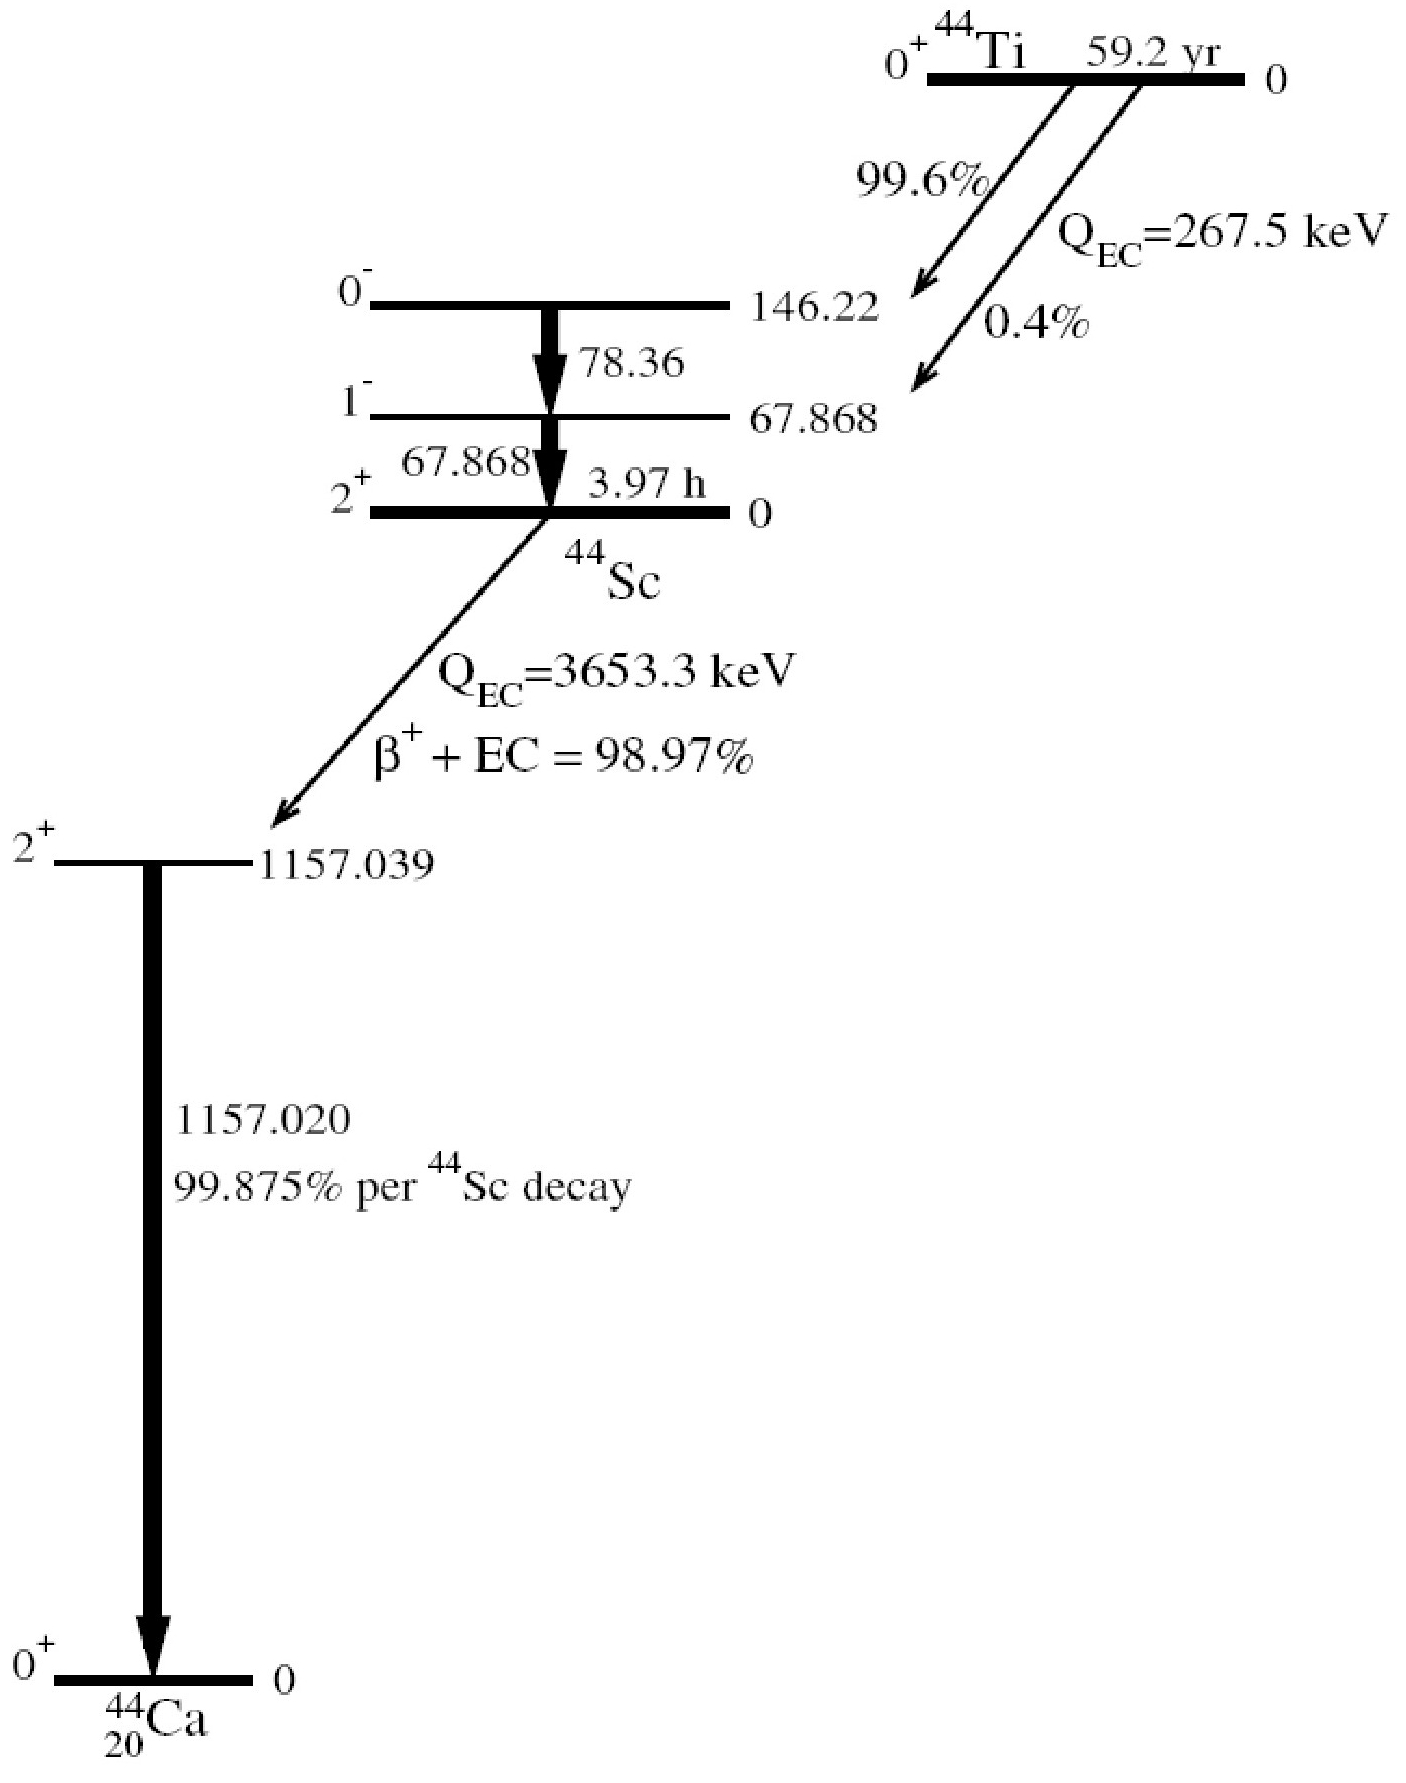
\includegraphics[width=0.6\linewidth]{img/44Ti-decay_reduziert}
			\caption{
			Reduziertes Zerfallsschema von Titan-44 über Scandium-44 zu Calcium-44. Zerfallswege geringer Wahrscheinlichkeit sind nicht dargestellt.
			\cite{Zerfallsschema} % theoretisch copyrightmäßig schwierig, weil ich den unnötigen Teil rausgecropt habe. Alternative: Anleitung scannen.
			}
			\label{fig_Zerfallsschema}
	\end{figure}


	\subsection{Beta-Plus-Zerfall}
	Wie oben beschrieben findet die folgende Kernreaktion statt:
	\begin{equation}
		\label{eq_beta-plus}
		 _{21}^{44}\text{Sc} \rightarrow _{20}^{44}\text{Ca} + \text{e}^+ + \nu_{\text{e}}
	\end{equation}
	Das dabei entstandene Positron wird durch Wechselwirkung mit dem Rest der Probe unter Aussendung von Bremsstrahlung abgebremst.
	Wenn es ausreichend stark abgebremst ist, kann es mit einem Elektron in der Probe das instabile Positronium bilden.
	Beim Positronium unterscheidet man je nach Spinausrichtung von Positron und Elektron in Parapositronium ($S=0$) und Orthopositronium ($S=1$).
	Aufgrund von Spin- und Impulserhaltung zerfällt Orthopositronium in eine ungerade Anzahl Photonen, die mindestens \num{3} beträgt.
	Aus analogen Gründen zerfällt Parapositronium eine gerade Anzahl Photonen, aber mindestens \num{2}.
	Da Zerfälle, die die Produktion einer geringeren Menge an Photonen voraussetzt, wahrscheinlicher sind, zerfällt Orthopositronium deutlich langsamer als Parapositronium.
	Gleichzeitig kann durch Umgebungswechselwirkung Orthopositronium in Parapositronium übergehen, was während der vergleichsweise langen Zerfallsdauer wahrscheinlich ist.
	Deswegen kann man sich in den folgenden Betrachtungen im Wesentlichen auf den Zerfall von Parapositronium in zwei Photonen mit einer Energie von \SI{511}{keV} beschränken.
	Außerdem ist anzumerken, dass die mittlere Lebensdauer von Parapositronium bei \SI{125}{ps} liegt, was im Vergleich zur erwarteten Lebensdauer des untersuchten $\gamma$-Niveaus verschwindend gering ist (\cite{Anleitung}).

	\subsection{Elektroneneinfang}
	Beim Elektroneneinfang findet aufgrund der Überlagerung der Wellenfunktionen von Hüllenelektronen und Kern im Kern die folgende Umwandlung statt:
	\begin{equation}
		\label{eq_elec_cap}
		\text{e}^- + \text{p} \rightarrow \text{n} + \nu_{\text{e}}
	\end{equation}
	Insofern ist der Elektroneneinfang unwahrscheinlicher als der Beta-Zerfall, da der Überlappe der Wellenfunktionen im Allgemeinen gering ist.
	Andererseits stellt er aber weniger strikte Anforderungen an die Zerfallsenergie.

	\subsection{Wechselwirkung der $\gamma$-Photonen mit Materie}

	Die bei den zuvor beschriebenen Zerfallsprozessen entstandenen Photonen können mit Kern oder Hüllenelektronen der Umgebung oder deren elektromagnetischen Feldern wechselwirken.
	Da die Wechselwirkung mit Atomkernen aufgrund des geringen Anteils des Kernvolumens am Atomvolumen einen deutlich geringeren Wirkungsquerschnitt hat, überwiegt die Wechselwirkung mit Hüllenelektronen.

	\subsubsection{Photoeffekt}
	Ein einfallendes $\gamma$-Photon kann im Atom absorbiert werden und die Emission eines Hüllenelektrons aus dem Atom heraus zufolge haben.
	Das herausgelöste Elektron erhält dabei die Differenz zwischen Energie des einfallenden Photons und der nötigen Ionisierungsenergie, um es aus dem Atom zu lösen.
	Auf das nun unbesetzte Energieniveau kann ein Elektron aus einer höheren Schale (oder ein freies Elektron) absinken, wobei ein Photon charakteristischer Energie (bei freien Elektronen kontinuierliches Spektrum ab einer Mindestenergie) frei wird. % das freie Elektron ist halt unwahrscheinlich, aber ich habs mal trotzdem erwähnt.

	\subsubsection{Compton-Effekt}
	Bei der Compton-Streuung überlebt im Gegensatz zum Photoeffekt das einfallende $\gamma$-Photon und bewegt sich danach im Allgemeinen mit geänderter Richtung und Energie. % lel, philosophisch, ob ein Quant anderer Quantenzahl 'das gleiche' Quant ist, also ob das Photon noch es selbst ist nach Frequenzänderung, imo nö, außer dem würden wir ja beim Messen auch einen Andern Prozess der Anfung und Ende gleich wie Compton hat als Compton betiteln, unabhängig ob es Compton war (==Terme höherer Ordnung)?
	Wenn die Energie des einfallenden Photons deutlich größer als die Ionisierungsenergie ist, kann das Hüllenelektron wie ein freies Elektron betrachtet werden.
	Die Energieänderung des Photons hängt dann nur vom Winkel der Richtungsänderung und seiner Ursprungsenergie ab.

	\subsubsection{Paarbildungseffekt}

	Hier wird im Coulomb-Feld eines Atomkerns ein $\gamma$-Photon in ein Positron und eine Elektron umgewandelt.
	Dies kann aufgrund von Energie- und Impulserhaltungssatz nur in Wechselwirkung mit einem Atomkern stattfinden.

	\subsection{Szintillator}

	Ein Szintillator ist ein Detektor, der einfallende Strahlung in eine einfacher messbare elektromagnetische Strahlung umwandelt.
	In diesem Versuch wurde ein anorganischer Halbleiter-Szintillator verwendet.
	Bei diesem wird durch die einfallende Strahlung ein Elektron aus den Valenzband in das Leitungsband angeregt und lässt im Valenzband ein Loch zurück.
	Wenn das Elektron an einer Störstelle mit dem Loch rekombiniert, kann dies durch die an der Störstelle modifizierten Bandstruktur schrittweise geschehen, weshalb Strahlung einer geringeren, leichter detektierbaren Wellenlänge frei wird.

	\subsection{Photomultiplier}

	In einem Photomultiplier werden einzelne einfallende Photonen in ein messbares Signal umgewandelt.
	Das Funktionsprinzip ist in \cref{fig_Photomultiplier} dargestellt.
	Dabei löst zunächst ein einfallendes Photon an der Kathode (negative Spannung) ein Elektron aus.
	Dieses Elektron wird in Richtung der Anode (positive Spannung) beschleunigt und schlägt auf dem Weg dorthin aus den Dynoden zusätzliche Elektronen heraus.
	An der Anode kommen dann ausreichend viele Elektronen an, um einen messbaren Rückfluss zur Kathode zu erzeugen (bzw. über einen Widerstand eine messbare Spannung).

	\begin{figure}[H]
			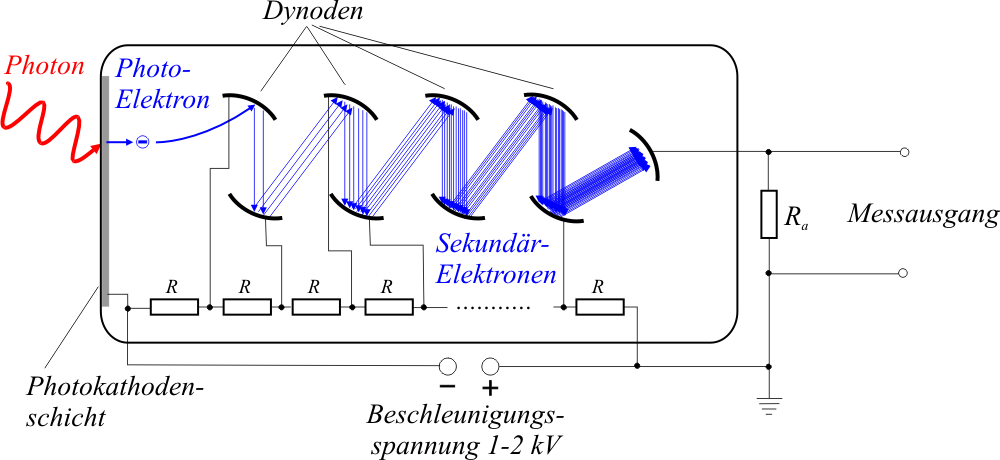
\includegraphics[width=0.6\linewidth]{img/Photomultiplier}
			\caption{
			Schematische Darstellung eines Photomultipliers.
			\cite{Photomultiplier}
			}
			\label{fig_Photomultiplier}
	\end{figure}

	\section{Methoden}
	% Bilder von der Website klauen
	% einer will Präsens
	Der Versuch wird in zwei Teilen durchgeführt und eine Titan-44-Probe untersucht.
	Zunächst wird der Zerfall des nach dem Beta-Zerfall entstehenden Positroniums genutzt, um eine Zeitkalibrierung zu ermöglichen.
	Dann wird die Zeitdifferenz der $\gamma$-Photonen der schrittweisen Abregung von Scandium-44 genutzt, um die Lebensdauer des mittleren Niveaus zu bestimmen.

	%Die eine Titan-44-Probe verlassende $\gamma$-Strahlung soll detektiert werden.
	%Zusätzlich soll die zeitliche Differenz zwischen zwei $\gamma$-Photonen eines bestimmten Energiefensters gemessen werden.

	Verwendet werden zwei Detektoren, die Szintillator und Photomultiplier kombinieren, um ein Signal zu erzeugen, das proportional zum einfallenden Photon ist.
	Diese werden mit Hochspannung (\SI{1400}{V} und \SI{1100}{V}) betrieben.
	Die Signale werden zunächst vorverstärkt und dann in einen Spektralverstärker geleitet.
	Dieser verstärkt das Signal einerseits zusätzlich und wandelt es in eine Form um, die später bei der Ermittlung der Zeitdifferenz Effekte von Walk und Jitter minimiert.
	Hierbei wird statt dem Überschreiten eines bestimmten Schwellenwerts der Nulldurchgang des näherungsweise sinusförmigen (eine Periode) Signals verwendet als zu vergleichender Zeitpunkt verwendet.
	Diese als fast Zero-Crossing bezeichnete Technik ist in \cref{fig_Zero-Cross} abgebildet.

	\begin{figure}[H]
			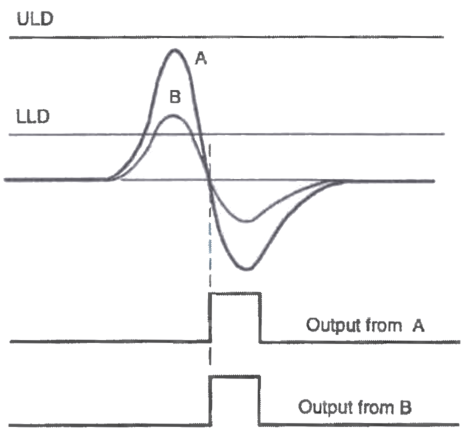
\includegraphics[width=0.6\linewidth]{img/Zero-Cross}
			\caption{
			Zero-Crossover SCA Output Triggering.
			\cite{Anleitung}
			}
			\label{fig_Zero-Cross}
	\end{figure}

	\subsection{Energiefilterung}

	Die Detektoren werden im \SI{180}{\degree}-Winkel zueinander auf die Probe gerichtet.
	Mit dem Aufbau bis zu diesem Punkt wird nun die Energie der Signale mit einem Multi Channel Analyzer in Kanäle aufgeteilt, digitalisiert und über einen Zeitraum von wenigen Minuten gemessen. %TODO ich bin mir nicht sicher, ob für das Energiegedöns das Signal schon umgeformt wurde...
	Die gemessenen Ereignisse werden dann über die entsprechenden Kanäle aufgetragen.
	In dem so gemessenen Energiespektrum wird der zum Zerfall des Positroniums gehörige Peak (\SI{511}{keV}) und der zur Abregung von Scandium-44 gehörige Peak (\SI{87,4}{keV} und \SI{67,8}{keV}) identifiziert und Anfang und Ende des Peaks im Kanalspektrum notiert.
	Über einen Dreisatz wird aus den Gesamtkanälen (8192) und dem möglichen Spannungsintervall (\SIrange{0}{10}{\volt}) der Signale der Spannungsbereich berechnet, in dem die Signale der Abregung und des Positroniumzerfalls liegen.
	Dies wird für beide Detektoren getrennt durchgeführt.

	\subsection{Zeitkalibrierung}
	Für diesen Versuchsteil der untersuchte Bereich auf den zum Positronium gehörigen Spannungsbereich begrenzt.
  Die übrigen Signale werden dann in einen Timing Single Channel Analyzer in ein Rechtecksignal konvertiert, wobei der Nulldurchgang für den Beginn des Rechtecksignals genutzt wird.
	Die Rechtecksignale von beiden Detektoren werden dann in einem Time to Amplitude Converter geleitet, der die zeitliche Differenz zwischen den Rechtecksignalen der beiden Detektoren in Ausgangssignal umwandelt, dessen Höhe proportional zur Zeitdifferenz ist.
	Dieses Signal wird dann vom Multichannel Analyzer digitalisiert und in Kanäle in Abhängigkeit von der Signalhöhe getrennt.
	Da die beiden Photonen vom Positronium im \SI{180}{\degree}-Winkel zeitgleich emittiert werden, kann nun der Zeitnullpunkt ermittelt werden, da hier das Maximum der gemessenen Ereignisse liegt.
	Die Zeitdifferenz aufgrund der Postion des Positroniums in der Probe wird hierbei vernachlässigt, da sie aufgrund der Bewegung der Photonen mit Lichtgeschwindigkeit verschwindend gering ist.

	Nun muss noch die Kanalbreite in eine Zeitdifferenz umgerechnet werden können.
	Hierfür wird anstelle der Detektoren ein Signalgenerator verwendet, der im Abstand vom \SI{640}{\nano \second} Signale erzeugt.
	Diese werden im Kanalspektrum aufgetragen und auf Basis des Mittelwerts der Abstände der Signale der Umrechnungsfaktor von Kanalbreite und Zeitdifferenz bestimmt.

	\subsection{Messung der mittleren Lebensdauer}

	Die Detektoren werden nun im \SI{90}{\degree}-Winkel zueinander auf die Probe gerichtet, um die Messung von Positronium auszuschließen und zusätzlich der Spannungsbereich nach dem Spektralverstärker auf den Bereich der Abregung von Scandium-44 begrenzt. %TODO eher Messung von korreliertem Positronium zu minimieren?
	Dann werden über \num{25} Stunden die auftretenden Ereignisse gemessen.
	Da diese die zeitlichen Differenzen zwischen Aussendung des Photons bei Abregung auf den mittleren angeregten Zustand und Abregung auf den Grundzustand darstellen, kann so die mittlere Lebensdauer des mittleren angeregten Zustands bestimmt werden.
	%  Zeiten
	% Zeitdifferenz: 25.3h
	% Positronium_Zeitdifferenz: 1.2h
	% Zeitkalibrierung: 7s
	% Energy_Start: 3.7m
	% Energy_Stop: 11.4m


	\section{Ergebnisse und Diskussion}
	%TODO Unsicherheiten


	%\subsection{Beobachtung und Datenanalyse}
	% Allgemeine Beobachtungen
	% Einflüsse von veränderten Parametern auf Messung
	% Berechung nach Aufgabenstellung
	\subsection{Unsicherheiten}
	In allen folgenden Graphen wurde die Unsicherheit bei $n_i$ Ereignissen mit $\sqrt{n_i}$ gemäß Poissonverteilung angegeben.
	%TODO dachte einmal für alle am Anfang ist einfacher. ggf mehr hier?

	\subsection{Energiespektren}
	Zuächst wurden die Energeispektren \cref{fig_energy_start} und \cref{fig_energy_stop} gemessen. Hieraus wurden die Kanalbereiche für aus dem jeweiligen Prozess stammende Photonen ermittelt.
	In Gelb wurde der $\gamma$-Peak gekennzeichnet und in lila der Positronium-Peak.
	Beim $\gamma$-Zerfall sind die Strahlungen der verschiedenen Niveaus nicht unterscheidbar aufgelösst (\SI{78.4}{keV} und \SI{67.8}{keV} \cite{Anleitung}). %TODO hier ggf. iwas warum die so sind?

	\begin{figure}[H]
		\centering
	\begin{subfigure}[b]{0.8\textwidth}
				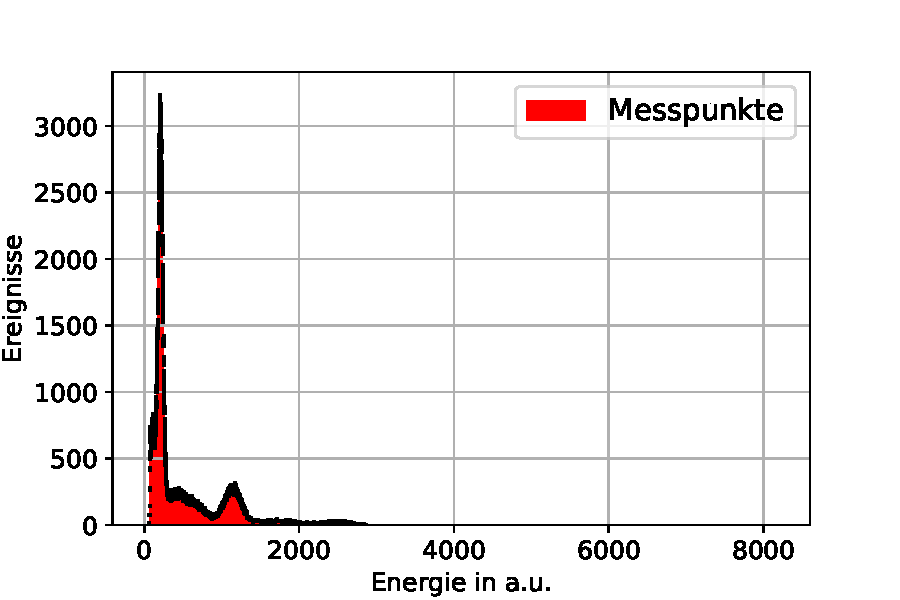
\includegraphics[width= 1 \linewidth]{img/Energiespektrum_Start}
				\caption{}
				\label{fig_energy_start}
		\end{subfigure}
	\begin{subfigure}[b]{0.8\textwidth}
				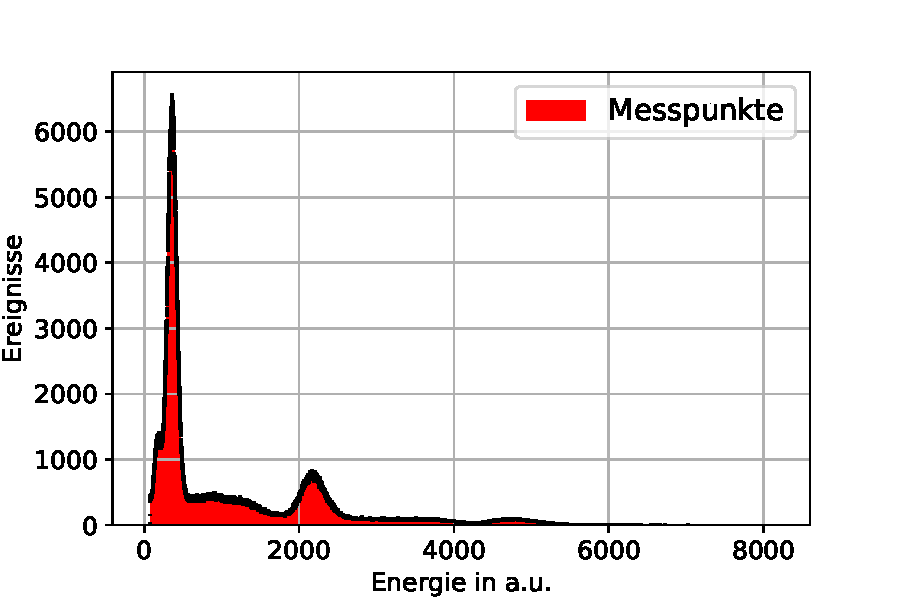
\includegraphics[width= 1 \linewidth]{img/Energiespektrum_Stop}
				\caption{}
				\label{fig_energy_stop}
		\end{subfigure}
		\caption{
				Energiespektren, welche von den zwei Messapparatur aufgenommen wurde.
				Die Energie ist in willkürlichen Einheiten angegeben, da nicht bekannt ist, welcher Photonenenergie der Multi Channel Analyzer welchen Kanal zuordnet, aber bekannt ist, dass ein höherer Kanal auch einer höheren Energie entspricht.
				Die Unsicherheiten sind in Schwarz abgebildet, sodass sich der Messwert mittig im schwarzen Bereich befindet.
				Die groben Grenzen des $\gamma$-Zerfall sind gelb und die des Positroniumzerfalls lila. %TODO grob hier fine?
				}
		\end{figure}

  \subsubsection{Zeitkalibrierung}\label{sss_zeitkali}
	Der Mittelwert der Abstände der Peaks in \cref{fig_zeitkalibrierung} beträgt \SI{514.8+-0.4}{}. Das heißt, so viele Kanäle entsprechen einer Zeit von \SI{640+-3}{ns}.

	%TODO kann man hier überhaupt mehr schreiben?
	\begin{figure}[H]
				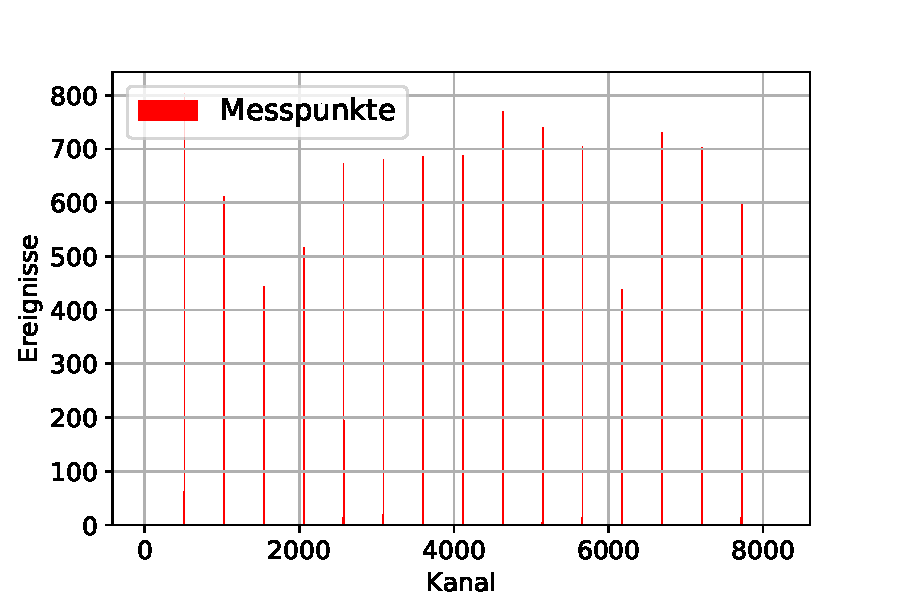
\includegraphics[width= 0.9 \linewidth]{img/Zeitkalibrierung}
				\caption{
				Zeitkalibrierung der Kanäle mittels eines Signalgenerators.
				Es gibt auch kleine Beiträge zu anderen Kanälen in naher Umgebung der Peaks, jedoch sind diese aufgrund der zu geringen Auflösung des Bildes kaum sichtbar.
				Die Unsicherheiten sind zur besseren Erkenntlichkeit nicht abgebildet.
				}
				\label{fig_zeitkalibrierung}
		\end{figure}

		\subsubsection{Bestimmung des Nullpunkts}
		In \cref{fig_positronium_zeitdifferenzen} sind die Messungen der Zeitdifferenzen des Positroniumzerfalls abgebildet.
		Da dieser sehr scharf ist, ist er in \cref{fig_positronium_zeitdifferenzen_zoom} vergrößert dargestellt.
		Es wird eine Gaußfunktion \ref{eq_gauss} an die Messpunkte angepasst:
		\begin{equation}
			\label{eq_gauss}
			%A * np.exp(-(x - x0)**2 / 2 / d**2)
			 f(t) = N\exp\left\{{\frac{(t-T_0)^2}{2 \Delta T^2}}\right\}
		\end{equation}
		Die Standardabweichung $\Delta T$ des Fits beschreibt für die folgende Bestimmung der Lebensdauer des $\gamma$-Niveaus die Unsicherheit der Messapparatur bei der Auflösung von Zeitdifferenzen, da beim Positroniumzerfall kein zeitlicher Unterschied vorliegt. %TODO ref in Theorie? bzw. vernachlässigbar klein

	\begin{figure}[H]
				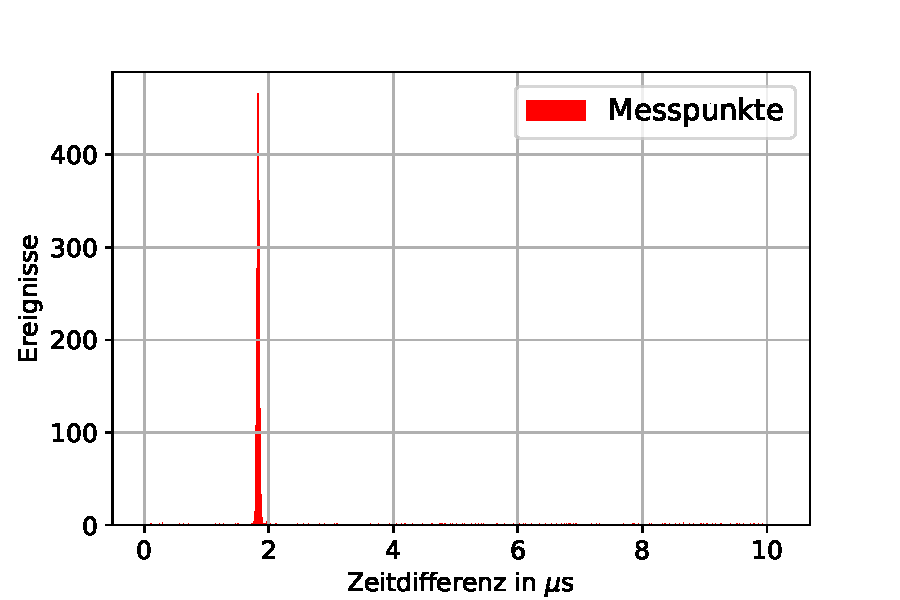
\includegraphics[width= 0.8 \linewidth]{img/Positronium_Zeitdifferenz}
				\caption{
				Zeitdifferenz zwischen den Photonen des Positroniumzerfalls.
				Die Unsicherheiten sind zur besseren Erkenntlichkeit nicht abgebildet.
				}
				\label{fig_positronium_zeitdifferenzen}
		\end{figure}

	\begin{figure}[H]
				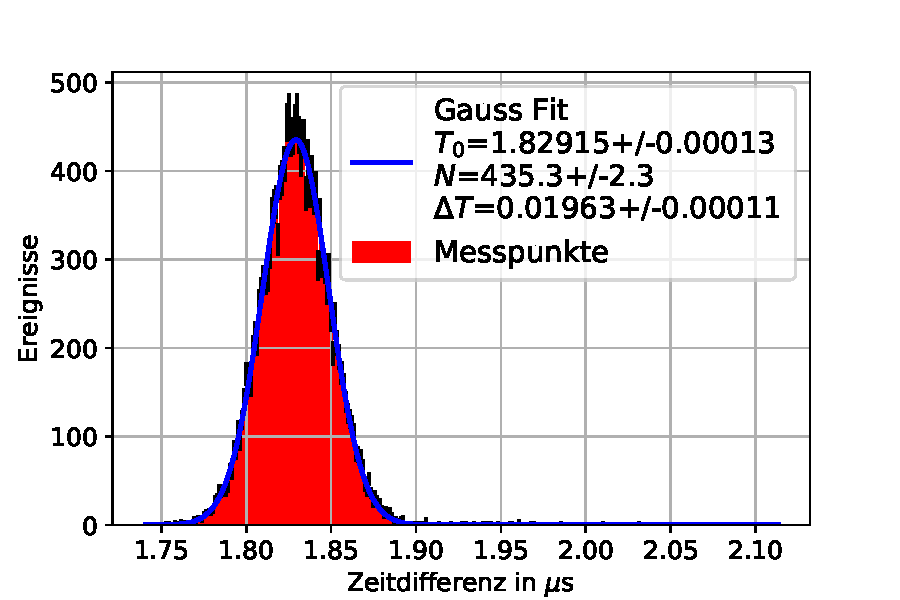
\includegraphics[width= 0.8 \linewidth]{img/Positronium_Zeitdifferenz_zoom}
				\caption{
				Vergrößertes Zeitdifferenzpeak zwischen den Photonen des Positroniumzerfalls.
				Die Unsicherheiten sind in Schwarz abgebildet, sodass sich der Messwert mittig im schwarzen Bereich befindet.
				Die blaue Kurve ist ein Gaußkurve nach \cref{eq_gauss}.
				}
				\label{fig_positronium_zeitdifferenzen_zoom}
		\end{figure}

		\subsubsection{Bestimmung der Lebensdauer}

		\subsubsection*{Abschätzung}
		Mit \cref{fig_zeitdifferenz_zoom} wurde die Halbwertszeit grob abgeschätzt.
		Hierbei beschreibt die grüne Horizontale bei \SI{125+-10}{} Ereignissen den Untergrund (siehe \cref{fig_zeitdifferenz}).
		In gelb verlaufen eine Horizontale und eine Vertikale durch das abgeschätzte Maximum.
		Ebenso sind die Punkte mit halb so vielen Ereignissen (ohne den Untergrund) lila markiert.
		Die Unsicherheit setzt sich aus der Unschärfe des Maximums und der Breite des Schnitts der lila Horizontalen mit den Messpunkten.
		Gegenüber diesen ist die Zeitunsicherheit aus \cref{sss_zeitkali} von \SI{0.02}{\mu s} vernachlässigbar.
		In \cref{tb_punkte} sind die geschätzten Punkte aufgeführt.
		Hierbei pflanzen sich die Unsicherheiten für Summen und Differenzen jeweils gemäß $\sigma=\sqrt{\sigma_1^2+\sigma_2^2}$ fort.
		Die Differenz der Zeitpunkte gibt die Halbwertszeit $t_{1/2}$ $\SI{149+-4}{ns}$ bzw. $\SI{151+-4}{ns}$.

		\begin{table}[H]
		\centering
		\begin{tabular}{c| c | c }
			 Farbe&$t$ in \SI{}{\mu s}&$N-$Untergrund\\ \hline
			 Gelb&\SI{1.75+-0.04}{}&\SI{424+-14}{}\\
			 Lila&\SI{1.89+-0.02}{}&\SI{212+-7}{}\\
			 Lila&\SI{1.59+-0.02}{}&\SI{212+-7}{}\\
		\end{tabular}
		\caption{
			Markierte Punkte aus \cref{fig_positronium_zeitdifferenzen_zoom}.
		}
			 \label{tb_punkte}
	\end{table}
		\begin{figure}[H]
				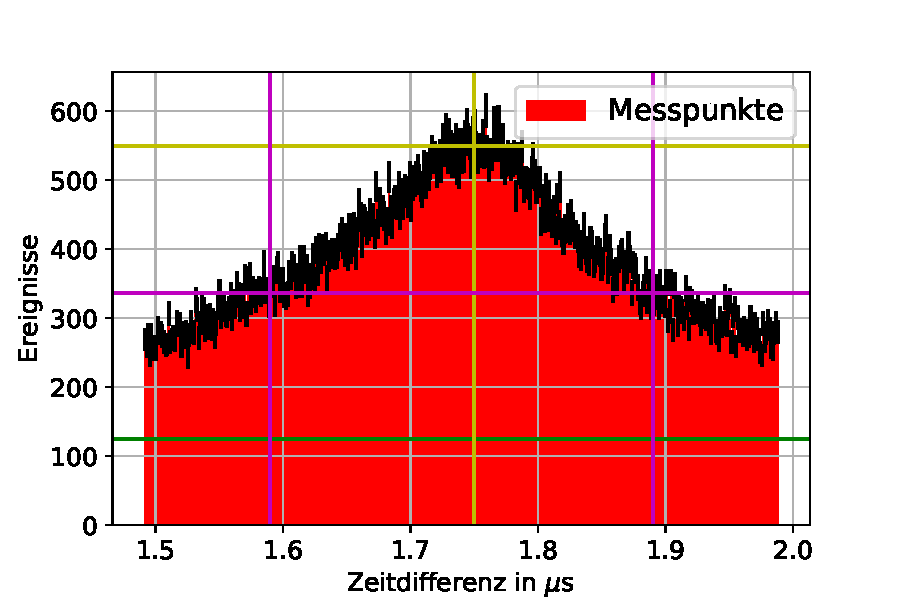
\includegraphics[width= 0.7 \linewidth]{img/Zeitdifferenzen_zoom}
				\caption{
				Vergrößerung um das Maximum der Zeitdifferenzen zwischen den Photonen der Gamma-Niveau-Abregung.
				Die Unsicherheiten sind in Schwarz abgebildet, sodass sich der Messwert mittig im schwarzen Bereich befindet.
				Die grüne Horizontale ist der Untergrund.
				In gelb und lila sind die Punkte, welche für die Abschätzung der Halbwertszeit verwendet werden, markiert.
				}
				\label{fig_zeitdifferenz_zoom}
		\end{figure}

		\subsubsection*{Fit}
		In \cref{fig_zeitdifferenz} ist die grüne Linie der Mittelwert aller Ereignisse bei einer Zeitdifferenz, die größer als \SI{4}{\mu s} ist.
		Somit beträgt der Untergrund \SI{120+-21}{} Ereignisse.
		Der lila Fit ist eine in die jeweilige Richtung exponentiell abfallende Funktion:
		\begin{equation}
			\label{eq_dexp}
			f(t)=N\cdot (\exp{\left\{-\lambda_3(t-T_0)\right\}}\Theta(t-T_0)+\exp{\left\{\lambda_4(t-T_0)\right\}}\Theta(T_0-t))
		\end{equation}
		Dabei ist $\Theta$ die Heaviside-Funktion.
	\begin{figure}[H]
				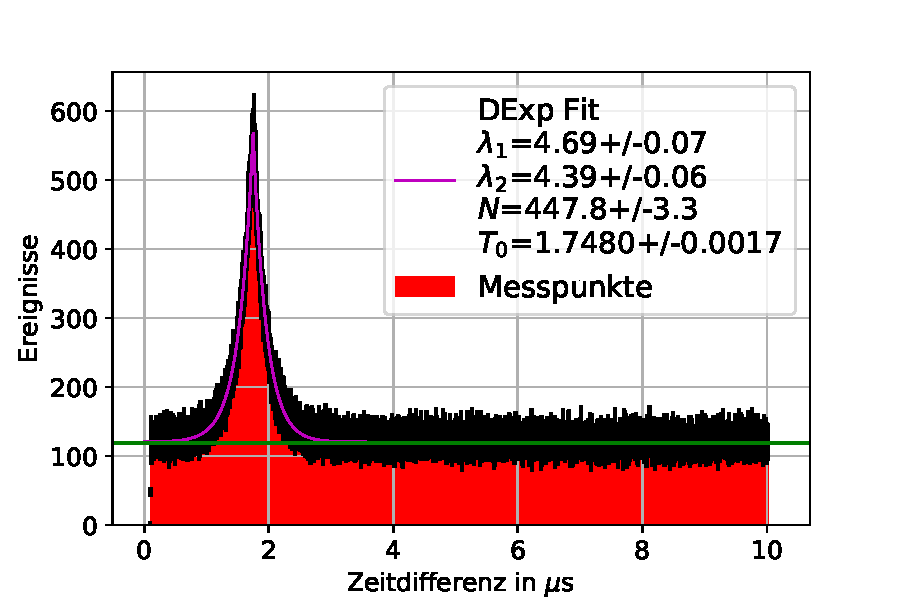
\includegraphics[width= 0.9 \linewidth]{img/Zeitdifferenzen}
				\caption{
				Zeitdifferenzen zwischen den Photonen der Gamma-Niveau-Abregung.
				Die Unsicherheiten sind in Schwarz abgebildet, sodass sich der Messwert mittig im schwarzen Bereich befindet.
				}
				\label{fig_zeitdifferenz}
		\end{figure}
		\subsubsection*{Mittelwert}
		Außerdem lässt sich die mittlere Lebensdauer durch
		\begin{equation}
			\label{eq_mittel}
			\tau = \frac{\sum_i t_i \cdot n_i}{\sum_i n_i}
		\end{equation}
		bestimmen.
		Wobei hier $t_i$ der Abstand zum Maximum (hier $\SI{1.74}{\mu s}$) und $n_i$ die Anzahl der Ereignisse \textbf{ohne} den Untergrund ist.
		\cref{eq_mittel} ist also der gewichtete und normierte Mittelwert der Lebensdauern und die Unsicherheit ergibt sich aus dem Quotienten der Standardabweichung und der Wurzel der Anzahl der Messpunkte über welche gemittelt wird ($\frac{s}{\sqrt{N}}$).

		Es folgt $\tau_5=\SI{229+-3}{ns}$ im Bereich von $\SI{1.74}{\mu s}$ bis $\SI{3}{\mu s}$ und umgekehrt in $\SI{0.4}{\mu s}$ bis $\SI{1.74}{\mu s}$ folgt $\tau_6=\SI{233+-4}{\mu s}$.
		Die Bereiche wurden so gewählt, da in \cref{eq_mittel} die Terme hoher $t_i$, die um Null schwanken, zu großen Fehlern führen.

		In \cref{tb_leb} sind die insgesamt resultierenden Lebensdauern aufgeführt.
		\begin{table}[H]
		\centering
		\begin{tabular}{c| c | c | c | c  }
			 Methode&Index&$\lambda$ in \si{\mu s^{-1}}& $\tau=1/\lambda$ in \si{ns} &$t_{1/2}=\tau\ln 2$ in \si{ns}\\ \hline
			 Halbwertsbreite&1&\SI{4.7+-0.12}{}&\SI{215+-6}{}&\SI{149+-4}{}\\
			 &2&\SI{4.6+-0.12}{}&\SI{217+-6}{}&\SI{151+-4}{}\\
			 &Mittelwert 1+2&\SI{4.65+-0.1}{}&\SI{216+-4}{}&\SI{150+-3}{}\\\hline
			 Fit&3&\SI{4.69+-0.07}{}&\SI{213+-3}{}&\SI{147+-2}{} \\
			 &4&\SI{4.39+-0.06}{}&\SI{228+-3}{}&\SI{158+-2}{} \\
			 &Mittelwert 3+4&\SI{4.54+-0.15}{}&\SI{220+-8}{}&\SI{150+-7}{}\\\hline
			 Mittelwert&5&\SI{4.37+-0.06}{}&\SI{229+-3}{}&\SI{159+-2}{}\\
			 &6&\SI{4.29+-0.07}{}&\SI{233+-4}{}&\SI{162+-3}{}\\
			 &Mittelwert 5+6&\SI{4.33+-0.06}{}&\SI{231+-3}{}&\SI{160+-3}{}\\\hline
		\end{tabular}
		\caption{
		Verschiedene gemessene Lebensdauern, bzw. Halbwertszeiten, des angeregten $\gamma$-Niveaus von $^{44}$Sc.
		}
			 \label{tb_leb}
	\end{table}
	\subsection{Diskussion}
	% Bezug/Nutzen oder sonst was
	% auch hier die Hypothese wiederholen
	% keine Messwerte hier, nach manchen Menschen, zumindest "direkt" erstellte Diagramme net hier, auch wenn Lesbarkeit-bla
	In den Energiespektren in \crefrange{fig_energy_start}{fig_energy_stop} wird dem höchsten Peak die Photonen aus der Abregung von Scandium-44 zugeordnet.
	Diese sind aufgrund des geringen Energieunterschieds von \SI{11}{keV} nicht unterscheidbar.
	Dem deutlich kleineren, aber immer noch ausgeprägten Peak bei höherer Energie werden die Photonen des Positroniumzerfalls bei \SI{511}{keV} zugeordnet.

	In \cref{fig_zeitdifferenz} ist zu erkennen, dass die Zeitdifferenzen symmetrisch um einen Peak herum gemessen werden. %TODO Naja der Fit ist nicht so schön symmetrisch.
	Dies liegt daran, dass negative Zeitdifferenzen dann auftreten, wenn das erste Photon am zweiten Detektor und dann das zweite Photon am ersten Detektor ankommt.
	Da keine ausgezeichnete Emissionsrichtung bei dem Zerfall existiert, ist dieser Fall ein genauso valider Messwert.
	Aufgrund der zeitlichen Verschiebung zwischen der Signalerzeugung und -verarbeitung der beiden Detektoren liegt der Peak allerdings nicht bei Null, sondern im positiven Bereich.
	Die Position des Peaks sollte dementsprechend bei demselben Wert liegen, der zuvor als Zeitnullpunkt (\cref{fig_positronium_zeitdifferenzen_zoom}) bestimmt wurde.
	Dies ist allerdings nicht der Fall.
	Aus der Messung des Positroniums ergibt sich ein Wert von \SI{1,8292+-0.00013}{\mu s}, während der Peak bei \SI{1,7480+-0.00017}{\mu s} liegt.
	Eine Erklärung für diesen Effekt bleiben wir hier schuldig, da sich lediglich die Ausrichtung der Detektoren geändert hat.


	\subsubsection{Vergleich der mittleren Lebensdauern}
	Beim Vergleich der in \cref{tb_leb} angegebenen mit verschiedenen Methoden bestimmten Lebensdauern stellt man fest, dass sich Werte ergeben, die teilweise um mehr als den doppelten Fehler voneinander abweichen.
	Wenn man den Literaturwert von \SI{216 \pm 4,2}{\nano s} (\cite{Anleitung}, Unsicherheit auf Basis mangelnder Nachkommastellen) zum Vergleich heranzieht, stellt man fest, dass die Ergebnisse einiger Methoden hiervon signifikant nach oben abweichen.
	Bei der Ermittlung mittels Fit ist außerdem auch ein signifikanter Unterschied zwischen den beiden Flanken festzustellen.
	Zu erwarten wäre hier eigentlich, dass die Ergebnisse innerhalb der Messunsicherheiten übereinstimmen.
	Dass dem nicht so ist, muss auf Untergrundeffekte und durch die Messapparatur verursachte systematische Fehler zurückgeführt werden.
	Dennoch liegen die Werte hinreichend nah beieinander, um eine Einschätzung über die mittlere Lebensdauer des untersuchten Zustands zuzulassen.

	\section{Schlussfolgerung}
	% Rückgriff auf Hypothese und drittes Nennen dieser
	Insgesamt gesehen lässt sich sagen, dass die Lebensdauer des untersuchten ersten angeregten $\gamma$-Niveaus in Scandium-44 erfolgreich bestimmt werden konnte.
	Der Vergleich der verschiedenen Methoden zur Bestimmung dieser führen jedoch zu Ergebnissen, die sich um mehr als die Messunsicherheiten unterscheiden.
	Um diese Effekte näher zu untersuchen, wäre ein längerer Messzeitraum ein erster Ansatz, da dies Aufschluss darauf geben könnte, ob es sich tatsächlich um systematische Fehler handelt.
	Nicht geklärt werden konnte, warum bei der Messung von Positronium-Photonen und Scandium-Photonen unterschiedliche Zeitdifferenzen auftreten.
	Um diesen Effekt näher zu untersuchen, wäre es hilfreich, die Messungen erneut durchzuführen, um festzustellen, ob er mit der Messung in unterschiedlichen Energienfenstern, bei verschiedenen Detektorarmwinkeln oder den unterschiedlichen Messzeitpunkten zusammenhängt.

	% Quellen zitieren, Websiten mit Zugriffsdatum
	% Verweise auf das Laborbuch (sind erlaubt)
	% Tabelle + Bilder mit Beschriftung
	\printbibliography %TODO Die Anleitung ist so irgendwie unschön gereferenced, aber was soll man machen...
\end{document}
